\documentclass[11pt,a4paper]{article}

\usepackage[utf8]{inputenc}
\usepackage[T1]{fontenc}
\usepackage[turkish,shorthands=off]{babel}
\usepackage[margin=2.5cm]{geometry}
\usepackage{listings}
\usepackage{booktabs}
\usepackage{graphicx}
\usepackage{xcolor}
\usepackage{hyperref}
\usepackage{pgfplots}
\usepackage{tikz}
\usetikzlibrary{shapes.geometric, arrows.meta, positioning, babel}
\usepackage{float}
\usepackage{enumitem}
\usepackage{tcolorbox}
\usepackage{amsmath}
\usepackage{fancyhdr}
\usepackage{needspace}

\lstdefinelanguage{json}{
    basicstyle=\ttfamily\tiny,
    stringstyle=\color{blue},
    string=[s]{"}{"},
    comment=[l]{//},
    morecomment=[s]{/*}{*/}
}
\lstdefinelanguage{markdown}{
    basicstyle=\ttfamily\tiny,
    keywords={#, ##, ###, ####},
    keywordstyle=\color{blue}\bfseries
}
\lstset{
  inputencoding=utf8,
  extendedchars=true,
  literate=
    {ı}{{\i}}1
    {İ}{{\.I}}1
    {ğ}{{\breve{g}}}1
    {Ğ}{{\breve{G}}}1
    {ü}{{\"u}}1
    {Ü}{{\"U}}1
    {ş}{{\c{s}}}1
    {Ş}{{\c{S}}}1
    {ö}{{\"o}}1
    {Ö}{{\"O}}1
    {ç}{{\c{c}}}1
    {Ç}{{\c{C}}}1
}

\pgfplotsset{compat=1.18}

\title{On-Premise LLM Tabanlı Doküman Analizi — Araştırma Raporu}
\author{Ediz Şentürk}
\date{\today}

\begin{document}
\shorthandoff{=!:}

\maketitle
\tableofcontents
\newpage

\section{Yönetici Özeti}
Tamamen yerel ve kapalı devre (on-premise) çalışan bir doküman analizi çözümü açık kaynaklı büyük dil modelleri kullanılarak başarıyla geliştirilmiştir. Sistem, PDF ayrıştırma işlemleri için Docling altyapısını; hızlı metadata çıkarımı için Phi-4-mini ve derinlemesine tablo/varlık (entity) analizi için Qwen 2.5 modellerinden oluşan Çift LLM (Dual LLM) mimarisini kullanmaktadır. Ayrıca Akıllı VLM (Görsel Dil Modeli) optimizasyonu sayesinde, metin tabanlı (native), taranmış (scanned) ve karma (mixed) PDF formatları sıfır harici API çağrısı ile işlenmekte ve standartlaştırılmış JSON çıktıları üretilmektedir.

\section{Teknoloji Araştırması ve Karşılaştırma}

\subsection{Yerel LLM'ler}
Araştırma kapsamında 9 farklı açık kaynaklı büyük dil modeli, doküman analizi görevinde karşılaştırmalı olarak değerlendirilmiştir. Tüm testlerde aynı fatura dokümanı ve aynı çıkarım prompt'u kullanılmıştır.

\begin{table}[H]
\centering
\caption{Yerel LLM Karşılaştırması}
\begin{tabular}{lcccccc}
\toprule
Model & Boyut & Hız (tok/s) & TTFT & Metadata & Tablo & Genel Not \\
\midrule
Phi-4-mini & 3.8B & 46.4 & Anında & Kusursuz & Mükemmel & A \\
Llama 3.1 & 8B & 84.9 & Anında & Kusursuz & \# Atladı & B+ \\
Llama 3.2 & 3B & 85.0 & Anında & Eksik & Mükemmel & C+ \\
Gemma 2 & 9B & 36.2 & Anında & Boş & Kesildi & D \\
Qwen 2.5-VL & 7B & 56.1 & 157s & Kusursuz & Mükemmel & F \\
Qwen 3 & 8B & 46.9 & 163s & Kusursuz & Mükemmel & F \\
Qwen 3.5 & 9B & 27.3 & 118s & Kusursuz & Mükemmel & F \\
DeepSeek R1 & 7B & 31.4 & 25s & Boş & Uydurma & F \\
Mistral v0.3 & 7B & 14.4 & Anında & Kırık & Doğru & F \\
\bottomrule
\end{tabular}
\end{table}

\begin{figure}[H]
\centering
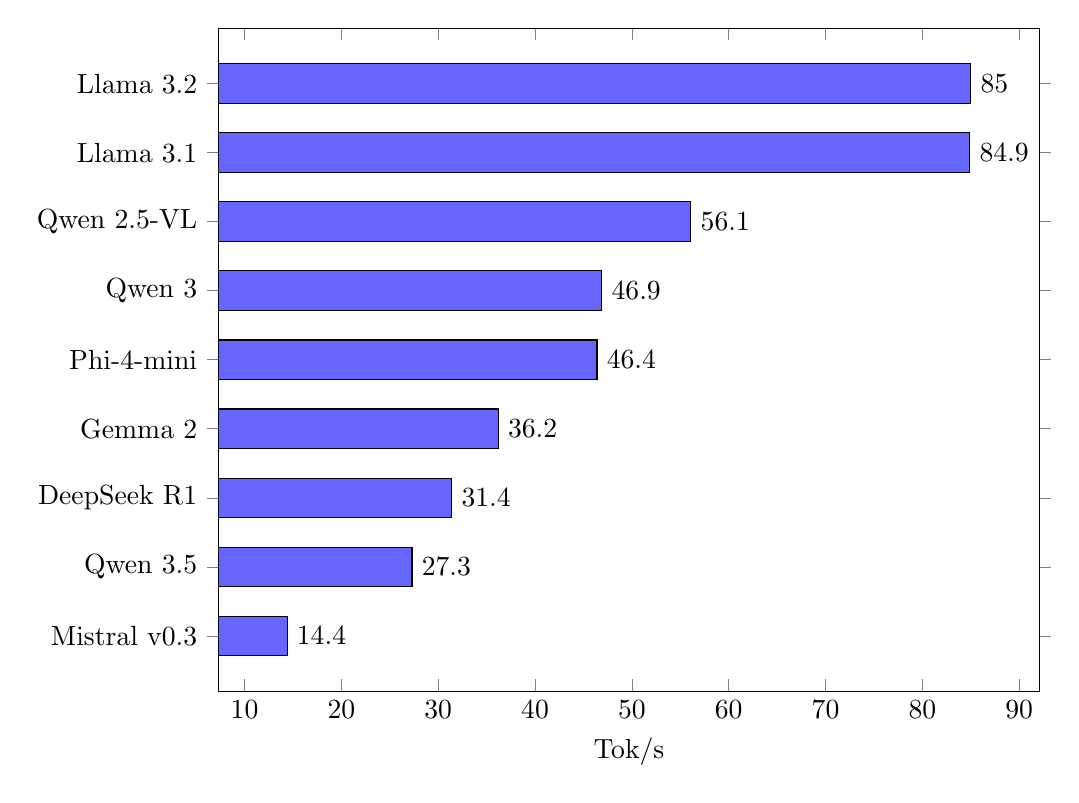
\begin{tikzpicture}
\begin{axis}[
    xbar,
    y dir=reverse,
    bar width=0.5cm,
    width=12cm,
    height=10cm,
    enlarge y limits=0.1,
    xlabel={Tok/s},
    symbolic y coords={{Llama 3.2},{Llama 3.1},{Qwen 2.5-VL},{Qwen 3},{Phi-4-mini},{Gemma 2},{DeepSeek R1},{Qwen 3.5},{Mistral v0.3}},
    ytick=data,
    nodes near coords,
    nodes near coords align={horizontal},
]
\addplot[fill=blue!60] coordinates {
    (85.0,{Llama 3.2})
    (84.9,{Llama 3.1})
    (56.1,{Qwen 2.5-VL})
    (46.9,{Qwen 3})
    (46.4,{Phi-4-mini})
    (36.2,{Gemma 2})
    (31.4,{DeepSeek R1})
    (27.3,{Qwen 3.5})
    (14.4,{Mistral v0.3})
};
\end{axis}
\end{tikzpicture}
\caption{Model Hız Karşılaştırması (tok/s)}
\end{figure}

\begin{figure}[H]
\centering
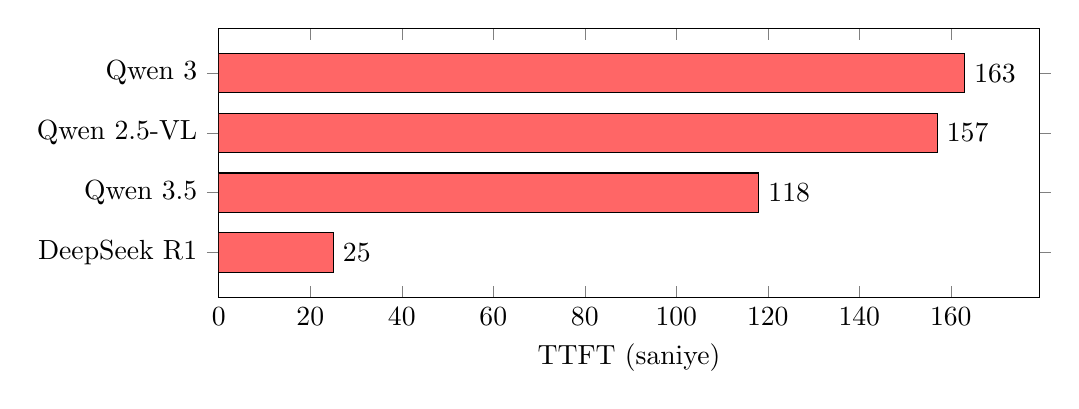
\begin{tikzpicture}
\begin{axis}[
    xbar,
    y dir=reverse,
    bar width=0.5cm,
    width=12cm,
    height=5cm,
    enlarge y limits=0.25,
    xlabel={TTFT (saniye)},
    symbolic y coords={{Qwen 3},{Qwen 2.5-VL},{Qwen 3.5},{DeepSeek R1}},
    ytick=data,
    nodes near coords,
    nodes near coords align={horizontal},
    xmin=0,
]
\addplot[fill=red!60] coordinates {
    (163,{Qwen 3})
    (157,{Qwen 2.5-VL})
    (118,{Qwen 3.5})
    (25,{DeepSeek R1})
};
\end{axis}
\end{tikzpicture}
\caption{İlk Token Süresi (TTFT) Yüksek Olan Modeller (Qwen modellerinde ilk token süresi 118s--163s iken; Phi-4-mini, Llama ve Gemma modelleri anında yanıt üretmektedir)}
\end{figure}

\begin{tcolorbox}[colback=yellow!10, colframe=orange!80, title=Önemli Uyarı]
Unsloth Studio beta sürümü, macOS ortamında Apple Metal (GPU) altyapısını tam kapasiteyle kullanamamaktadır. Bu nedenle raporlanan token üretim hızları, donanımın gerçek performans kapasitesini yansıtmayabilir. Metal desteği olgunlaştığında daha yüksek throughput değerleri beklenmektedir.
\end{tcolorbox}

\needspace{10\baselineskip}
\subsubsection{Model Seçim Gerekçesi}
Benchmark sonuçlarında hiçbir tek modelin tüm kriterlerde üstünlük sağlayamadığı görülmüştür. \textbf{Phi-4-mini} hız ve TTFT'de lider iken tablo/entity çıkarımında sınırlı kalabilmektedir. \textbf{Qwen 2.5} ise tablo ve entity doğruluğunda kusursuza yakın performans sergilerken, tek başına kullanıldığında TTFT 157 saniyeyi bulmaktadır.

Bu nedenle \textbf{Çift LLM Hibrit Mimarisi} benimsenmiştir:
\begin{itemize}[noitemsep]
\item \textbf{Phi-4-mini (Phase 1):} Metadata, özet ve key-value çıkarımı — hızlı ilk yanıt
\item \textbf{Qwen 2.5 (Phase 2-3):} Tablo ve entity çıkarımı — yüksek doğruluk
\end{itemize}
Bu mimari, tek model yaklaşımının güçlü yönlerini birleştirirken zayıf yönlerini kompanse etmektedir.

\subsection{Görsel Dil Modelleri (VLM)}
Qwen2.5-VL, Qwen3-VL, LLaVA ve InternVL modelleri değerlendirilmiştir. Görselden tablo verisi çıkarma konusundaki yüksek doğruluğu, yerleşik Ollama desteği ve 8B parametrelik verimliliği nedeniyle Qwen 2.5-VL tercih edilmiştir. Bu model, taranmış dokümanlarda OCR atlayıp doğrudan veri çıkarımında en iyi başarıyı sunmuştur.

\begin{table}[H]
\centering
\caption{VLM Karşılaştırması}
\begin{tabular}{lllc}
\toprule
Model & Parametre & Tablo Çıkarımı & Ollama Desteği \\
\midrule
Qwen 2.5-VL & 7B & Mükemmel & Var \\
Qwen 3-VL & 8B & Çok İyi & Beta \\
LLaVA & 7B/13B & Yetersiz & Var \\
InternVL & 8B & İyi & Yok (Sınırlı) \\
\bottomrule
\end{tabular}
\end{table}

\subsection{OCR Çözümleri}
Farklı OCR motorları hız ve dil desteği bağlamında analiz edilmiştir. Docling'in yerleşik RapidOCR boru hattı sayesinde çoğu durumda harici bir OCR çözümüne ihtiyaç duyulmamaktadır.

\begin{table}[H]
\centering
\caption{OCR Motorları Karşılaştırması}
\begin{tabular}{llcll}
\toprule
Çözüm & Dil Desteği & Hız & Lisans & Notlar \\
\midrule
Azure OCR & Mükemmel & Hızlı & Ticari (On-Prem) & Yüksek lisans maliyeti \\
Tesseract & Çok İyi & Yavaş & Apache 2.0 & Klasik, standart \\
EasyOCR & İyi & Orta & Apache 2.0 & GPU gerektirir \\
RapidOCR & İyi & Çok Hızlı & Apache 2.0 & \textbf{Docling içinde yerleşik} \\
ocrmac & Yalnızca Apple & Hızlı & Yere Özel & macOS kısıtlı \\
\bottomrule
\end{tabular}
\end{table}

\subsection{Doküman Ayrıştırma Araçları}
Araştırılan doküman ayrıştırma kütüphaneleri aşağıda listelenmiştir. Docling, layout (düzen) koruma, tablo çıkarımı ve yerleşik OCR entegrasyonu kabiliyetlerini tek pakette sunduğu için ana parser olarak seçilmiştir.

\begin{table}[H]
\centering
\caption{Doküman Ayrıştırma (Parsing) Araçları}
\begin{tabular}{lccccc}
\toprule
Araç & Layout Koruma & Tablo Çıkarım & BBox Desteği & OCR & Lisans \\
\midrule
Docling & Mükemmel & Mükemmel & Var & Var & MIT \\
Marker & İyi & İyi & Yok & Kısmi & GPL \\
MinerU & Çok İyi & Orta & Var & Kısmi & Apache \\
Unstructured & Orta & Orta & Kısmi & Var & Apache \\
PyMuPDF & Düşük & Yetersiz & Var & Yok & AGPL \\
PDFPlumber & Düşük & İyi & Var & Yok & MIT \\
\bottomrule
\end{tabular}
\end{table}

\section{Sistem Mimarisi}

\subsection{Pipeline Genel Görünümü}
\begin{figure}[H]
\centering
\resizebox{0.98\textwidth}{!}{%
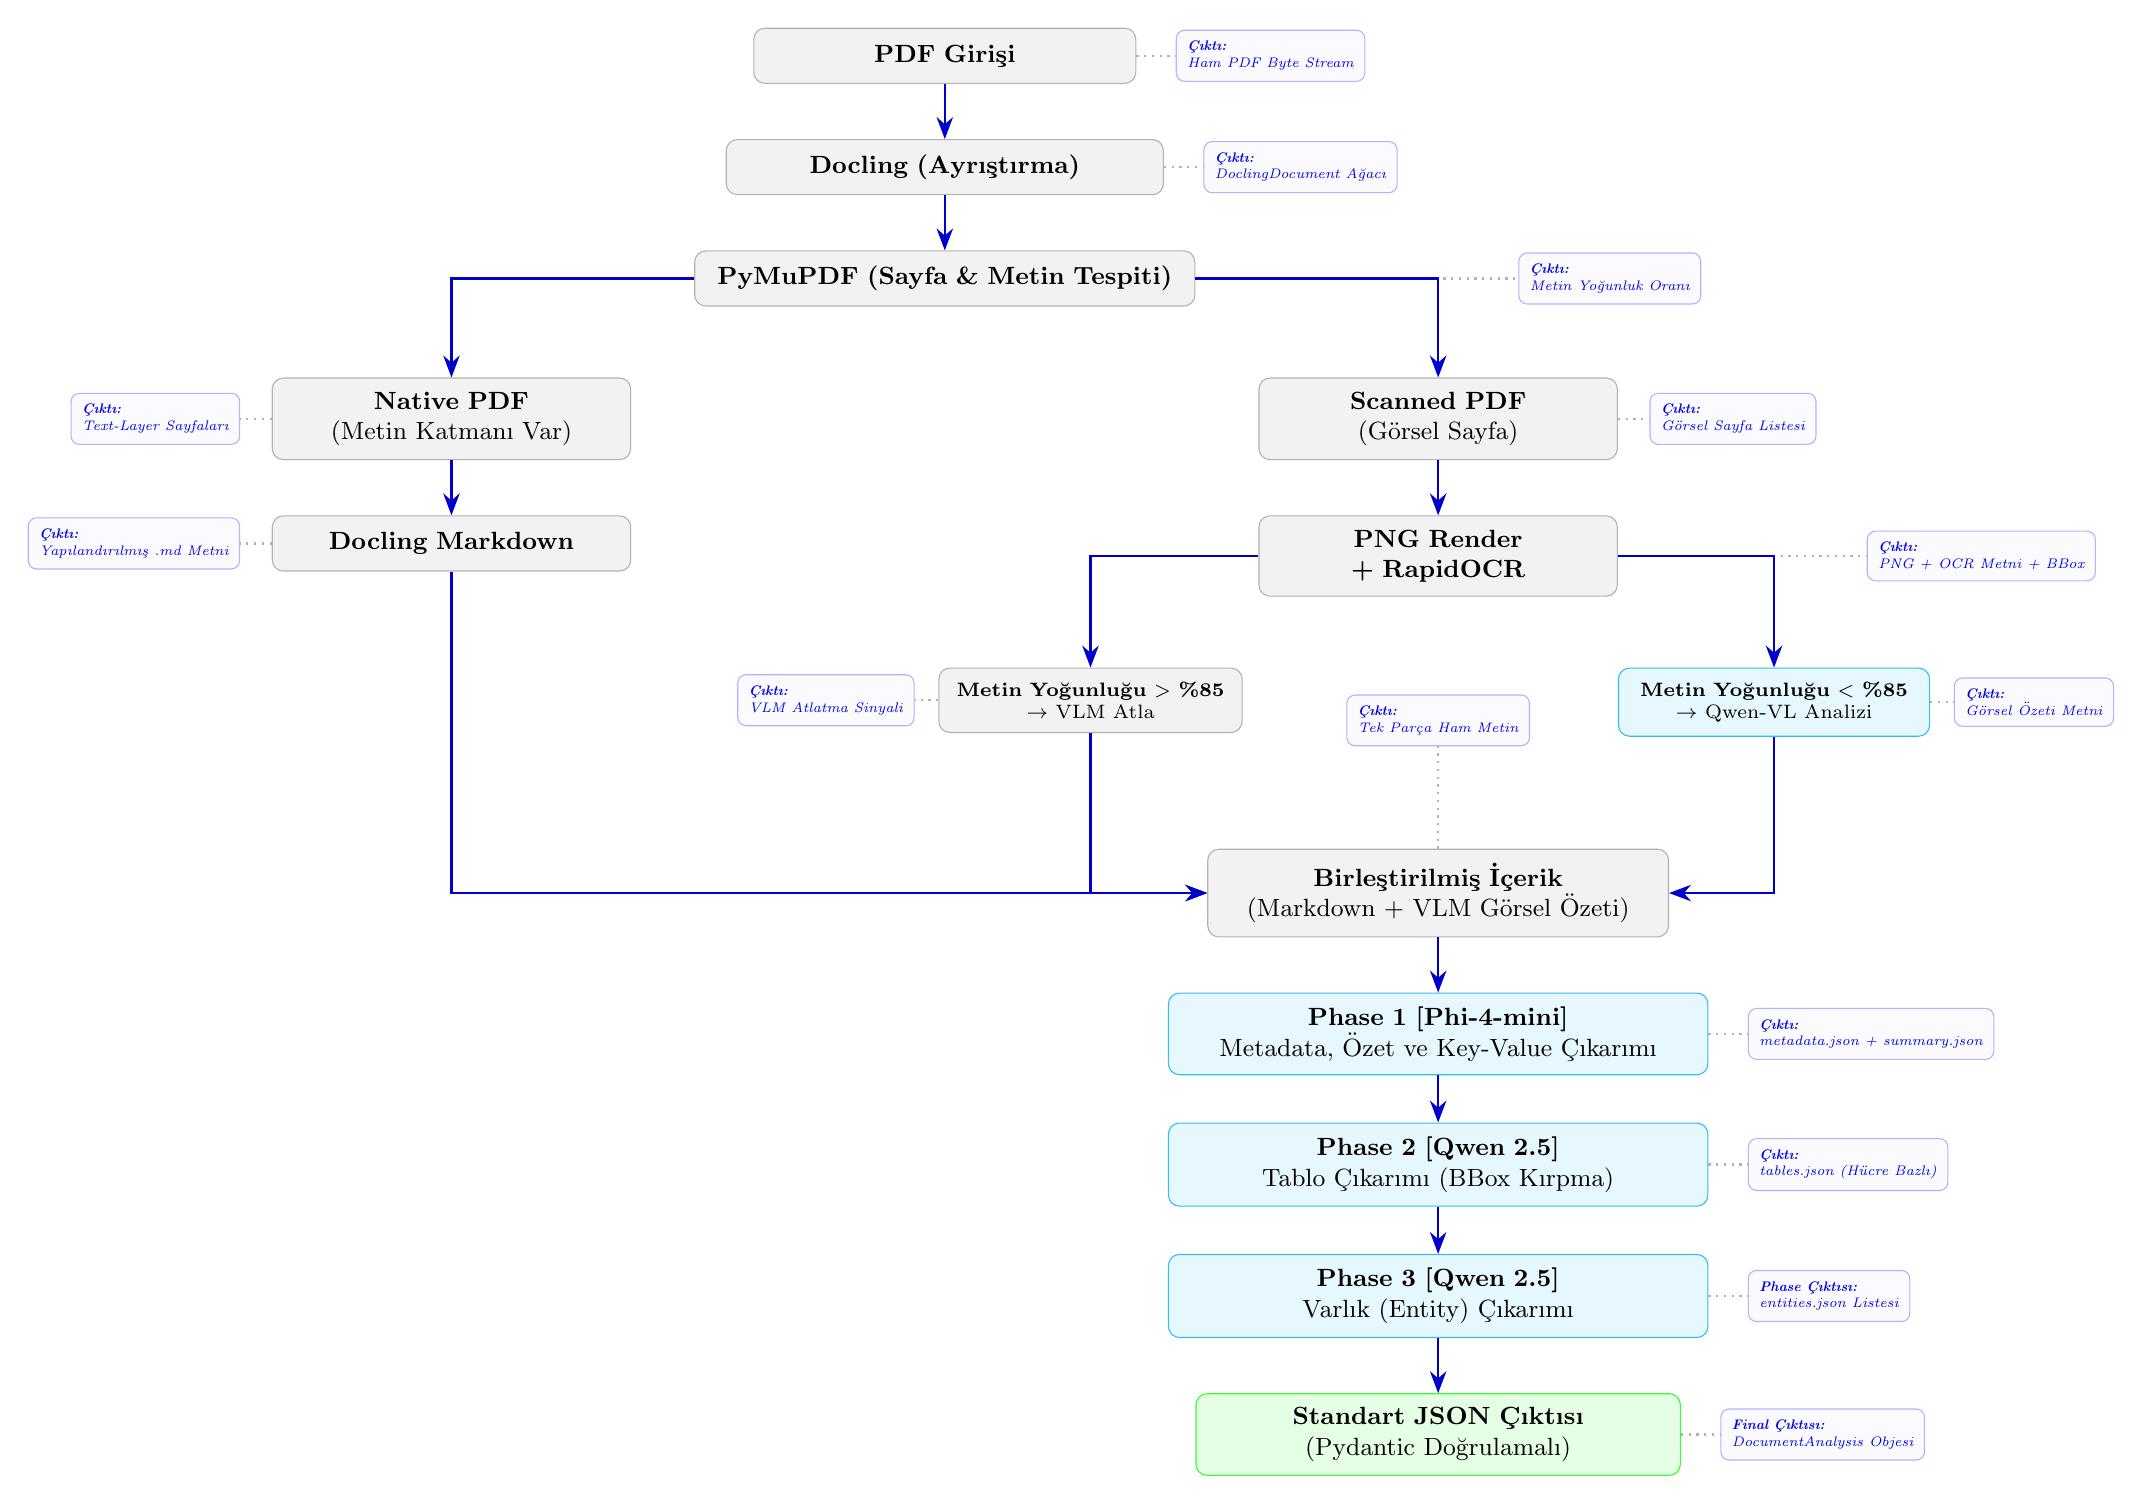
\begin{tikzpicture}[
    box/.style={rectangle, draw=blue!60, fill=blue!5, rounded corners, align=center, minimum height=0.7cm, font=\small, inner sep=5pt},
    model/.style={rectangle, draw=cyan!80, fill=cyan!10, rounded corners, align=center, minimum height=0.7cm, font=\small, inner sep=5pt},
    output/.style={rectangle, draw=green!80, fill=green!10, rounded corners, align=center, minimum height=0.7cm, font=\small, inner sep=5pt},
    process/.style={rectangle, draw=gray!60, fill=gray!10, rounded corners, align=center, minimum height=0.7cm, font=\small, inner sep=5pt},
    outtag/.style={rectangle, draw=blue!30, fill=blue!2, rounded corners=3pt, font=\tiny\itshape, text=blue!90!black, inner sep=4pt, align=left},
    arrow/.style={-{Stealth[scale=1.2]}, thick, draw=blue!80!black},
    side/.style={dotted, draw=gray!60, thick}
]

% Ana İşlem Kutuları (Ortalanmış ve Yan Dallı)
\node[process, text width=4.5cm] (input) {\textbf{PDF Girişi}};
\node[process, below=0.7cm of input, text width=5.2cm] (docling) {\textbf{Docling (Ayrıştırma)}};
\node[process, below=0.7cm of docling, text width=6.0cm] (pymupdf) {\textbf{PyMuPDF (Sayfa \& Metin Tespiti)}};

\node[process, below left=0.9cm and 0.8cm of pymupdf, text width=4.2cm] (native) {\textbf{Native PDF}\\ (Metin Katmanı Var)};
\node[process, below right=0.9cm and 0.8cm of pymupdf, text width=4.2cm] (scanned) {\textbf{Scanned PDF}\\ (Görsel Sayfa)};

\node[process, below=0.7cm of native, text width=4.2cm] (mdout) {\textbf{Docling Markdown}};
\node[process, below=0.7cm of scanned, text width=4.2cm] (render) {\textbf{PNG Render + RapidOCR}};

\node[process, below left=0.9cm and 0.2cm of render, font=\scriptsize, text width=3.5cm] (vlm_skip) {\textbf{Metin Yoğunluğu $>$ \%85}\\ $\rightarrow$ VLM Atla};
\node[model, below right=0.9cm and 0cm of render, font=\scriptsize, text width=3.6cm] (vlm_run) {\textbf{Metin Yoğunluğu $<$ \%85}\\ $\rightarrow$ Qwen-VL Analizi};

\node[process, below=3.2cm of render, text width=5.5cm] (combined) {\textbf{Birleştirilmiş İçerik}\\ (Markdown + VLM Görsel Özeti)};

\node[model, below=0.7cm of combined, text width=6.5cm] (phase1) {\textbf{Phase 1 [Phi-4-mini]}\\ Metadata, Özet ve Key-Value Çıkarımı};
\node[model, below=0.6cm of phase1, text width=6.5cm] (phase2) {\textbf{Phase 2 [Qwen 2.5]}\\ Tablo Çıkarımı (BBox Kırpma)};
\node[model, below=0.6cm of phase2, text width=6.5cm] (phase3) {\textbf{Phase 3 [Qwen 2.5]}\\ Varlık (Entity) Çıkarımı};

\node[output, below=0.7cm of phase3, text width=5.8cm] (json) {\textbf{Standart JSON Çıktısı}\\ (Pydantic Doğrulamalı)};

% YAN ÇIKTI ETİKETLERİ (Kutucukların Yanına Eklenen Çıktılar)
\node[outtag, right=0.5cm of input] (o_input) {\textbf{Çıktı:}\\ Ham PDF Byte Stream};
\node[outtag, right=0.5cm of docling] (o_docling) {\textbf{Çıktı:}\\ DoclingDocument Ağacı};
\node[outtag, right=4.10cm of pymupdf] (o_pymupdf) {\textbf{Çıktı:}\\ Metin Yoğunluk Oranı};

\node[outtag, left=0.4cm of native] (o_native) {\textbf{Çıktı:}\\ Text-Layer Sayfaları};
\node[outtag, right=0.4cm of scanned] (o_scanned) {\textbf{Çıktı:}\\ Görsel Sayfa Listesi};

\node[outtag, left=0.4cm of mdout] (o_mdout) {\textbf{Çıktı:}\\ Yapılandırılmış .md Metni};
\node[outtag, right=3.16cm of render] (o_render) {\textbf{Çıktı:}\\ PNG + OCR Metni + BBox};

\node[outtag, left=0.3cm of vlm_skip] (o_vlm_skip) {\textbf{Çıktı:}\\ VLM Atlatma Sinyali};
\node[outtag, right=0.3cm of vlm_run] (o_vlm_run) {\textbf{Çıktı:}\\ Görsel Özeti Metni};

\node[outtag, above=1.30cm of combined] (o_combined) {\textbf{Çıktı:}\\ Tek Parça Ham Metin};
\node[outtag, right=0.5cm of phase1] (o_phase1) {\textbf{Çıktı:}\\ metadata.json + summary.json};
\node[outtag, right=0.5cm of phase2] (o_phase2) {\textbf{Çıktı:}\\ tables.json (Hücre Bazlı)};
\node[outtag, right=0.5cm of phase3] (o_phase3) {\textbf{Phase Çıktısı:}\\ entities.json Listesi};
\node[outtag, right=0.5cm of json] (o_json) {\textbf{Final Çıktısı:}\\ DocumentAnalysis Objesi};

% Yan Etiket Bağlantıları
\draw[side] (input) -- (o_input);
\draw[side] (docling) -- (o_docling);
\draw[side] (pymupdf) -- (o_pymupdf);
\draw[side] (native) -- (o_native);
\draw[side] (scanned) -- (o_scanned);
\draw[side] (mdout) -- (o_mdout);
\draw[side] (render) -- (o_render);
\draw[side] (vlm_skip) -- (o_vlm_skip);
\draw[side] (vlm_run) -- (o_vlm_run);
\draw[side] (combined) -- (o_combined);
\draw[side] (phase1) -- (o_phase1);
\draw[side] (phase2) -- (o_phase2);
\draw[side] (phase3) -- (o_phase3);
\draw[side] (json) -- (o_json);

% Ana Akış Akış Okları
\draw[arrow] (input) -- (docling);
\draw[arrow] (docling) -- (pymupdf);

\draw[arrow] (pymupdf) -| (native);
\draw[arrow] (pymupdf) -| (scanned);

\draw[arrow] (native) -- (mdout);
\draw[arrow] (scanned) -- (render);

\draw[arrow] (render) -| (vlm_skip);
\draw[arrow] (render) -| (vlm_run);

\draw[arrow] (mdout) |- (combined);
\draw[arrow] (vlm_skip) |- (combined);
\draw[arrow] (vlm_run) |- (combined);

\draw[arrow] (combined) -- (phase1);
\draw[arrow] (phase1) -- (phase2);
\draw[arrow] (phase2) -- (phase3);
\draw[arrow] (phase3) -- (json);

\end{tikzpicture}%
}
\caption{Doküman İşleme Boru Hattı ve Veri Çıktıları (Pipeline Architecture)}
\end{figure}

\subsubsection{Native PDF Veri Akışı ve Aşamalara Göre Çıktı Örnekleri (native.pdf)}
Metin katmanına sahip belgeler doğrudan Docling ile ayrıştırılır. Metin yoğunluğu \%85'in üzerinde olduğu için VLM aşaması bypass edilir.

\vspace{4pt}\noindent\textbf{1. Docling Ayrıştırma Çıktısı (DoclingDocument $\rightarrow$ Markdown):}\par\vspace{2pt}
\begin{lstlisting}[language=markdown, basicstyle=\ttfamily\tiny, frame=single, breaklines=true, xleftmargin=0pt, xrightmargin=0pt]
# ACME CORPORATION
123 Business Avenue, Suite 456, New York, NY 10001
INVOICE INV-2025-00742 | Date: January 15, 2025 | Due Date: February 14, 2025
Bill To: Global Tech Solutions Ltd. (Attn: John Smith)

| # | Description | Qty | Unit Price | Amount |
| 1 | Cloud Infrastructure Setup | 1 | $4,500.00 | $4,500.00 |
| 2 | Custom API Development | 80 hrs | $150.00/hr | $12,000.00 |
Subtotal: $24,000.00 | Tax (8.5%): $2,040.00 | Total Due: $24,840.00
\end{lstlisting}

\vspace{4pt}\noindent\textbf{2. Phase 1 [Phi-4-mini] Çıktısı (Metadata \& Özet JSON):}\par\vspace{2pt}
\begin{lstlisting}[language=json, basicstyle=\ttfamily\tiny, frame=single, breaklines=true, xleftmargin=0pt, xrightmargin=0pt]
{
  "document_type": "invoice",
  "metadata": {
    "title": "ACME Corporation Invoice",
    "date": "January 15, 2025",
    "parties": ["ACME Corporation", "Global Tech Solutions Ltd."],
    "reference_numbers": ["INV-2025-00742", "PO-2025-1234"]
  },
  "summary": "Invoice for Cloud Infrastructure Setup and Custom API Development.",
  "key_values": [
    {"key": "Payment Terms", "value": "Net 30", "confidence": 1.0},
    {"key": "Total Due", "value": "$24,840.00", "confidence": 1.0}
  ]
}
\end{lstlisting}

\needspace{14\baselineskip}
\vspace{4pt}\noindent\textbf{3. Phase 2 [Qwen 2.5] Çıktısı (Hücre Bazlı Tablo JSON):}\par\vspace{2pt}
\begin{lstlisting}[language=json, basicstyle=\ttfamily\tiny, frame=single, breaklines=true, xleftmargin=0pt, xrightmargin=0pt]
{
  "tables": [
    {
      "caption": "Items & Services",
      "headers": ["#", "Description", "Qty", "Unit Price", "Amount"],
      "rows": [
        ["1", "Cloud Infrastructure Setup", "1", "$4,500.00", "$4,500.00"],
        ["2", "Custom API Development", "80 hrs", "$150.00/hr", "$12,000.00"],
        ["3", "Database Migration Service", "1", "$3,200.00", "$3,200.00"]
      ]
    }
  ]
}
\end{lstlisting}

\vspace{4pt}\noindent\textbf{4. Phase 3 [Qwen 2.5] Çıktısı (Varlık / Entity Listesi JSON):}\par\vspace{2pt}
\begin{lstlisting}[language=json, basicstyle=\ttfamily\tiny, frame=single, breaklines=true, xleftmargin=0pt, xrightmargin=0pt]
{
  "entities": [
    {"type": "organization", "value": "ACME CORPORATION"},
    {"type": "organization", "value": "Global Tech Solutions Ltd."},
    {"type": "person", "value": "John Smith"},
    {"type": "email", "value": "billing@acmecorp.com"},
    {"type": "amount", "value": "$24,840.00"}
  ]
}
\end{lstlisting}

\needspace{16\baselineskip}
\subsubsection{Mixed PDF Veri Akışı ve Aşamalara Göre Çıktı Örnekleri (mixed.pdf)}
Hem dijital metin hem taranmış görsel içeren belgelerde sayfa bazlı kontrol yapılır. Sayfa 1 ve 3 native işlenirken, taranmış olan Sayfa 2 için Qwen 2.5-VL görsel özeti üretilir.

\vspace{4pt}\noindent\textbf{1. VLM Görsel Analiz Çıktısı (Sayfa 2 Qwen 2.5-VL):}\par\vspace{2pt}
\begin{lstlisting}[language=markdown, basicstyle=\ttfamily\tiny, frame=single, breaklines=true, xleftmargin=0pt, xrightmargin=0pt]
[VLM Page 2 Analysis]
Visual Elements: Quarterly Performance Chart and Signed Approval Stamp.
Extracted Form Fields:
- Manager Approval: Approved (Sign: J. Smith, Date: 2025-01-18)
- Department: Cloud Operations & Infrastructure
\end{lstlisting}

\vspace{4pt}\noindent\textbf{2. Birleştirilmiş İçerik ve Çift LLM Çıktısı (Phase 1-3 JSON):}\par\vspace{2pt}
\begin{lstlisting}[language=json, basicstyle=\ttfamily\tiny, frame=single, breaklines=true, xleftmargin=0pt, xrightmargin=0pt]
{
  "document_type": "report",
  "metadata": {
    "title": "Quarterly Performance Report",
    "parties": ["Cloud Operations & Infrastructure"],
    "reference_numbers": ["QPR-2025-Q1"]
  },
  "key_values": [
    {"key": "Manager Approval", "value": "Approved", "confidence": 0.95}
  ],
  "entities": [
    {"type": "person", "value": "J. Smith"},
    {"type": "date", "value": "2025-01-18"}
  ]
}
\end{lstlisting}

\needspace{16\baselineskip}
\subsubsection{Scanned PDF Veri Akışı ve Aşamalara Göre Çıktı Örnekleri (scanned.pdf)}
Taranmış veya görsel tabanlı belgelerde metin yoğunluğu \%85'in altında olduğu için boru hattı 200 DPI PNG render ve RapidOCR/Qwen 2.5-VL görsel analiz moduna geçer.

\vspace{4pt}\noindent\textbf{1. PNG Render + RapidOCR ve VLM Çıktısı (BBox \& OCR):}\par\vspace{2pt}
\begin{lstlisting}[language=markdown, basicstyle=\ttfamily\tiny, frame=single, breaklines=true, xleftmargin=0pt, xrightmargin=0pt]
[Rendered 200 DPI Image -> RapidOCR Text + BBox & Qwen 2.5-VL]
Text Extracted: INVOICE INV-2025-00742 TOTAL DUE $24,840.00
Table BBox Cropped Region: [x: 54, y: 320, w: 504, h: 210] -> table_crop_1_0.png
VLM Table Extraction: Markdown grid generated from cropped image.
\end{lstlisting}

\needspace{16\baselineskip}
\vspace{4pt}\noindent\textbf{2. Scanned Doküman Tam JSON Çıktısı (Phase 1-3 Matrisi):}\par\vspace{2pt}
\begin{lstlisting}[language=json, basicstyle=\ttfamily\tiny, frame=single, breaklines=true, xleftmargin=0pt, xrightmargin=0pt]
{
  "document": {
    "source_file": "scanned.pdf",
    "pipeline_used": "ocr",
    "ocr_engine": "rapidocr"
  },
  "metadata": {
    "title": "Scanned Document Invoice",
    "reference_numbers": ["INV-2025-00742"]
  },
  "tables": [
    {
      "caption": "Scanned Invoice Items",
      "headers": ["Item", "Qty", "Price"],
      "rows": [["Cloud Setup", "1", "$4,500.00"]]
    }
  ]
}
\end{lstlisting}

\subsection{Çift LLM Mimarisi}
Sistem, hızı ve doğruluğu dengelemek amacıyla iki farklı dil modelini senkronize kullanmaktadır. Phase 1 aşamasında kullanılan \textbf{Phi-4-mini (3.8B)}, anında tepki süresi (TTFT) sayesinde metadata ve anahtar-değer (key-value) ikililerini saniyeler içinde çıkarabilmektedir. 

Tablo verileri ve karmaşık yapısal varlıkların (entities) çıkarımı gibi yoğun akıl yürütme gerektiren işler ise Phase 2 ve Phase 3 aşamalarında \textbf{Qwen 2.5 (7.6B)} modeline devredilmektedir. Bu sayede her iki modelin en güçlü yönlerinden faydalanılmaktadır.

Ollama üzerinde \texttt{OLLAMA\_MAX\_LOADED\_MODELS=3} parametresi kullanılarak modellerin sürekli RAM'e yüklenip silinmesi (model swap) önlenmiştir. Toplamda yaklaşık 7.5 GB RAM kullanılarak, 16 GB belleğe sahip standart bir Mac üzerinde bile sorunsuz ve yüksek performanslı çalışabilmesi sağlanmıştır.

\subsection{Akıllı VLM Optimizasyonu}
Taranmış dokümanlarda VLM maliyetini ve gecikmesini en aza indirmek için Akıllı VLM Optimizasyonu (Smart VLM) geliştirilmiştir.

\textbf{BBox tabanlı tablo kırpma:} Docling tarafından tespit edilen tablo koordinatları (BBox) kullanılarak, Pillow kütüphanesi yardımıyla sadece tablonun bulunduğu bölge kırpılır ve VLM'e tam sayfa yerine sadece ilgili bölge gönderilir.

\textbf{Text density bazlı VLM bypass:} PyMuPDF ile sayfanın metin yoğunluğu hesaplanır. Eğer sayfanın yüzde 85'ten fazlası makine tarafından okunabilir metin (native) içeriyorsa, VLM aşaması atlanarak (bypass) doğrudan markdown çıktısı üzerinden ilerlenir ve işlem süresi dramatik oranda kısaltılır.

\textbf{Adaptive resizing:} VLM'e gönderilecek görseller, çözünürlüklerini korurken bellek sınırlarını aşmamak adına dinamik olarak maksimum 1024x1024 piksel olacak şekilde yeniden boyutlandırılır.

\needspace{6\baselineskip}
\subsection{Streaming ve Parçalı Çıkarım}
Kullanıcı deneyimini iyileştirmek amacıyla çıkarım işlemi üç ayrı faza bölünmüştür. Her fazda Ollama'ya ayrı bir istek gönderilir ve sonuçlar anlık olarak (streaming) kullanıcıya aktarılır. Bu sayede kullanıcı, tüm analiz tamamlanmadan ilk anlamlı veriyi (metadata) $\sim$12 saniyede görebilir.

\needspace{16\baselineskip}
\section{Standart JSON Şeması}
Çıktılar tamamen standartlaştırılmış ve tip güvenliği Pydantic ile garanti altına alınmış bir JSON şemasına uymaktadır.

\begin{lstlisting}[language=json, basicstyle=\ttfamily\small, frame=single, breaklines=true]
{
  "document": {
    "source_file": "string",
    "page_count": "int",
    "document_type": "invoice|report|form|...",
    "language": "ISO code",
    "processing": { "pipeline_used", "model", "duration_seconds" }
  },
  "metadata": { "title", "date", "parties": [], "reference_numbers": [] },
  "summary": "string",
  "key_values": [{ "key", "value", "confidence" }],
  "tables": [{ "caption", "headers": [], "rows": [[]] }],
  "entities": [{ "type", "value" }],
  "raw_text_markdown": "string"
}
\end{lstlisting}

Yukarıdaki yapı, üst verilerden (metadata) tablolara (tables), varlıklara (entities) ve ham metne (raw\_text\_markdown) kadar genişletilebilir bir formattadır. Kurum içi sistemlere entegrasyonu kolaylaştırmak için modüler olarak tasarlanmıştır. Her alan isteğe bağlıdır (\texttt{Optional}); yeni alanlar mevcut şemayı bozmadan eklenebilir.

\needspace{32\baselineskip}
\subsection{Örnek JSON Çıktısı}
Aşağıda native PDF analizinden elde edilen gerçek çıktının özeti verilmiştir:

\begin{lstlisting}[basicstyle=\ttfamily\scriptsize, frame=single, breaklines=true]
{
  "document": {
    "source_file": "native.pdf",
    "page_count": 2,
    "document_type": "invoice",
    "processing": {
      "pipeline_used": "native",
      "model": "phi4-mini + qwen2.5:latest",
      "duration_seconds": 61.85
    }
  },
  "metadata": {
    "date": "January 15, 2025",
    "parties": ["Global Tech Solutions Ltd.", "ACME Corporation"],
    "reference_numbers": ["INV-2025-00742", "PO-2025-1234"]
  },
  "key_values": [
    {"key": "Subtotal", "value": "$24,000.00", "confidence": 1.0},
    {"key": "Tax (8.5%)", "value": "$2,040.00", "confidence": 1.0},
    {"key": "Total Due", "value": "$24,840.00", "confidence": 1.0}
  ],
  "tables": [{ "headers": ["#","Description","Qty","Unit Price","Amount"],
    "rows": [["1","Cloud Infrastructure Setup","1","$4,500","$4,500"], ...]
  }],
  "entities": [
    {"type": "person", "value": "John Smith"},
    {"type": "email", "value": "billing@acmecorp.com"}, ...
  ]
}
\end{lstlisting}

\section{Kavram Kanıtı (PoC)}

\subsection{Sistem Gereksinimleri}

\begin{table}[H]
\centering
\caption{Minimum ve Önerilen Sistem Gereksinimleri}
\resizebox{\textwidth}{!}{%
\begin{tabular}{llll}
\toprule
Bileşen & Minimum (Mac) & Önerilen (Mac) & PC / Sunucu (Win/Linux) \\
\midrule
İşletim Sistemi & macOS 14+ & macOS 15+ & Windows 11 / Ubuntu 22.04+ \\
İşlemci (CPU) & Apple M1 & Apple M2 Pro/Max & AMD Ryzen 7/9 veya Threadripper \\
Ekran Kartı (GPU) & Tümleşik Metal GPU & Tümleşik Metal GPU & NVIDIA RTX 4080/4090 (16-24GB VRAM) \\
Sistem RAM & 16 GB & 32 GB & 32 GB--64 GB DDR5 \\
Disk Alanı & 20 GB boş & 40 GB boş & 50 GB NVMe SSD \\
Python & 3.12+ & 3.12+ & 3.12+ \\
\bottomrule
\end{tabular}%
}
\end{table}

\subsection{Adım 1: Ollama Kurulumu}

Ollama, yerel LLM modellerini yönetmek ve çalıştırmak için kullanılan ana runtime'dır.

\begin{lstlisting}[language=bash, basicstyle=\ttfamily\small, frame=single, breaklines=true, caption={Ollama Kurulumu}]
# macOS icin (Homebrew ile)
brew install ollama

# Linux icin
curl -fsSL https://ollama.com/install.sh | sh

# Kurulumu dogrula
ollama --version
# Beklenen cikti: ollama version is 0.9.x
\end{lstlisting}

\subsection{Adım 2: Model İndirme}

Sistem üç adet model kullanmaktadır. İndirme süreleri internet hızına bağlı olarak 5-15 dakika arasında değişebilir.

\begin{lstlisting}[language=bash, basicstyle=\ttfamily\small, frame=single, breaklines=true, caption={Model İndirme}]
# Phase 1 - Hizli metadata modeli (2.5 GB)
ollama pull phi4-mini

# Phase 2-3 - Derin analiz modeli (4.7 GB)
ollama pull qwen2.5:latest

# VLM - Gorsel analiz modeli (6.0 GB)
ollama pull qwen2.5vl:7b
\end{lstlisting}

\needspace{10\baselineskip}
İndirilen modelleri doğrulamak için:

\begin{lstlisting}[language=bash, basicstyle=\ttfamily\small, frame=single, breaklines=true, caption={Model Doğrulama}]
# Indirilen modelleri listele
ollama list

# Beklenen cikti:
# NAME              SIZE
# phi4-mini:latest  2.8 GB
# qwen2.5:latest    4.6 GB
# qwen2.5vl:7b      6.0 GB
\end{lstlisting}

\needspace{14\baselineskip}
\subsection{Adım 3: Proje Kurulumu}

Proje, \texttt{uv} paket yöneticisi ile kurulmaktadır. \texttt{uv} mevcut değilse önce kurulmalıdır.

\begin{lstlisting}[language=bash, basicstyle=\ttfamily\small, frame=single, breaklines=true, caption={Proje Kurulumu}]
# uv paket yoneticisi kurulumu (yoksa)
curl -LsSf https://astral.sh/uv/install.sh | sh

# Projeyi klonla
git clone <repo-url>
cd wyseye-research-task

# Bagimliliklari kur (sanal ortam otomatik olusturulur)
uv sync

# Kurulumu dogrula
uv run docanalyze --help
\end{lstlisting}

\needspace{16\baselineskip}
\subsection{Adım 4: Çift Model Yapılandırması (Önerilen)}

Varsayılan olarak Ollama aynı anda yalnızca bir model tutar. Çift LLM mimarisinden tam performans almak için birden fazla modelin eşzamanlı olarak RAM'de tutulması gerekir. Bu yapılandırma model geçişlerindeki 3-5 saniyelik bekleme süresini ortadan kaldırır.

\begin{lstlisting}[language=bash, basicstyle=\ttfamily\small, frame=single, breaklines=true, caption={Çift Model Yapılandırması}]
# Yontem 1: Mevcut Ollama sunucusunu durdur ve yeniden baslat
pkill ollama
OLLAMA_MAX_LOADED_MODELS=3 OLLAMA_KEEP_ALIVE=30m ollama serve &

# Yontem 2: macOS'ta kalici ortam degiskeni
launchctl setenv OLLAMA_MAX_LOADED_MODELS 3
# Ardindan Ollama uygulamasini yeniden baslat
\end{lstlisting}

\begin{tcolorbox}[colback=blue!5, colframe=blue!60, title=RAM Bütçesi Hesaplaması]
\begin{itemize}[noitemsep]
\item \texttt{phi4-mini}: $\sim$2.8 GB
\item \texttt{qwen2.5:latest}: $\sim$4.6 GB
\item \textbf{Toplam}: $\sim$7.4 GB (16 GB RAM'de 8.6 GB boş kalır)
\item VLM dahil: $\sim$13.4 GB (32 GB RAM önerilir)
\end{itemize}
\end{tcolorbox}

\needspace{18\baselineskip}
\subsection{Adım 5: Modelleri Isıtma (Pre-warm)}

İlk analizden önce modellerin RAM'e yüklenmesini sağlamak için kısa bir ısıtma isteği gönderilebilir. Bu adım, ilk çalıştırmadaki cold-start gecikmesini ortadan kaldırır.

\begin{lstlisting}[language=bash, basicstyle=\ttfamily\small, frame=single, breaklines=true, caption={Model Isıtma}]
# phi4-mini'yi RAM'e yukle
curl -s http://localhost:11434/api/chat \
  -d '{"model":"phi4-mini","messages":[{"role":"user","content":"hi"}],"stream":false,"options":{"num_predict":1}}'

# qwen2.5'i RAM'e yukle
curl -s http://localhost:11434/api/chat \
  -d '{"model":"qwen2.5:latest","messages":[{"role":"user","content":"hi"}],"stream":false,"options":{"num_predict":1}}'

# Aktif modelleri dogrula
curl -s http://localhost:11434/api/ps | python3 -m json.tool

# Beklenen cikti:
# phi4-mini:latest     2.8 GB (VRAM)
# qwen2.5:latest       4.6 GB (VRAM)
\end{lstlisting}

\needspace{14\baselineskip}
\subsection{Adım 6: İlk Analizi Çalıştırma}

\begin{lstlisting}[language=bash, basicstyle=\ttfamily\small, frame=single, breaklines=true, caption={Doküman Analizi Çalıştırma}]
# Native PDF analizi
uv run docanalyze analyze samples/native.pdf

# Taranmis PDF analizi
uv run docanalyze analyze samples/scanned.pdf

# Karma PDF analizi
uv run docanalyze analyze samples/mixed.pdf

# Detayli log ile calistirma
uv run docanalyze analyze samples/native.pdf -v

# Cikti dosyasini belirtme
uv run docanalyze analyze samples/native.pdf -o sonuc.json
\end{lstlisting}

Başarılı bir çalıştırma sonrasında aşağıdaki gibi bir çıktı beklenir:

\begin{lstlisting}[basicstyle=\ttfamily\scriptsize, frame=single, breaklines=true, caption={Beklenen Çıktı Örneği}]
+-- On-Premise LLM Document Analyzer --+
| Input:  samples/native.pdf           |
| Fast: phi4-mini | Deep: qwen2.5      |
| Mode: Dual LLM Streaming + Chunked   |
+---------------------------------------+
Phase 1/3: Metadata & Key-Values  [12.5s]
Phase 2/3: Tables                 [17.2s]
Phase 3/3: Entities               [23.1s]
+-- Results --+
| Type: invoice | Tables: 1 | KV: 7   |
| Entities: 18  | Duration: 61.9s      |
| Saved to: outputs/native.json        |
+---------------------------------------+
\end{lstlisting}

\subsection{CLI Parametreleri}
\begin{table}[H]
\centering
\caption{CLI Komut Parametreleri}
\begin{tabular}{lll}
\toprule
Parametre & Varsayılan & Açıklama \\
\midrule
\texttt{--fast-model, -f} & phi4-mini & Phase 1 hızlı model \\
\texttt{--deep-model, -d} & qwen2.5:latest & Phase 2-3 derin model \\
\texttt{--vlm-model} & qwen2.5vl:7b & Görsel analiz modeli \\
\texttt{--output, -o} & outputs/<isim>.json & Çıktı dosya yolu \\
\texttt{--verbose, -v} & false & Detaylı log \\
\texttt{--stream/--no-stream} & true & Streaming modu \\
\bottomrule
\end{tabular}
\end{table}

\needspace{20\baselineskip}
\section{Performans Analizi}

\subsection{Pipeline Benchmark Sonuçları}
Farklı tipteki dokümanlar üzerinde yapılan ölçümler aşağıda listelenmiştir.

\begin{table}[H]
\centering
\caption{Benchmark Sonuçları}
\begin{tabular}{lcccccccc}
\toprule
Test & Toplam Süre & Parse & Phase 1 & Phase 2 & Phase 3 & Tablo & Entity & KV \\
\midrule
Native PDF & 61.9s & 8.9s & 12.5s & 17.2s & 23.1s & 1/1 & 18 & 7 \\
Scanned PDF & 154.5s & 86.8s & 19.7s & 28.2s & 19.8s & 1/1 & 15 & 9 \\
Mixed PDF & 126.9s & 60.1s & 12.1s & 30.2s & 24.4s & 2/2 & 21 & 3 \\
\bottomrule
\end{tabular}
\end{table}

\begin{figure}[H]
\centering
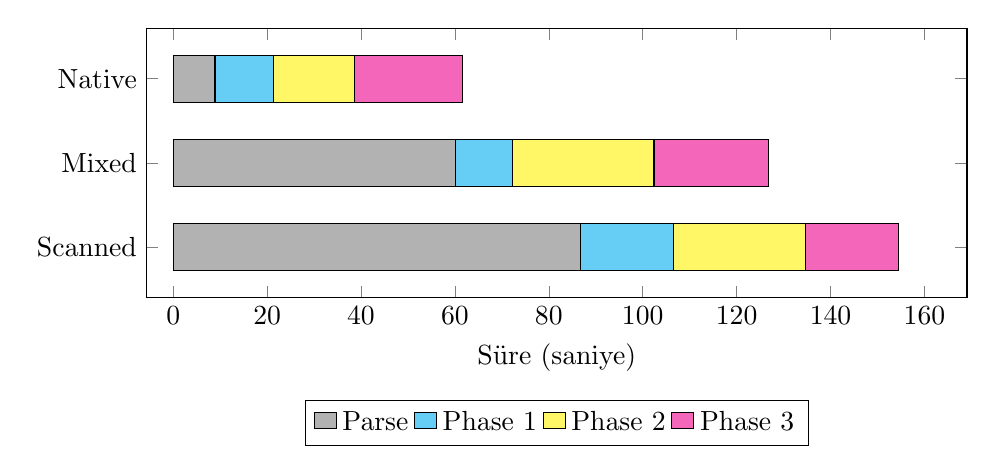
\begin{tikzpicture}
\begin{axis}[
    xbar stacked,
    y dir=reverse,
    bar width=0.6cm,
    width=12cm,
    height=5cm,
    enlarge y limits=0.3,
    xlabel={Süre (saniye)},
    symbolic y coords={{Native},{Mixed},{Scanned}},
    ytick=data,
    legend style={at={(0.5,-0.38)}, anchor=north, legend columns=-1}
]
\addplot[fill=gray!60] coordinates {(8.9,{Native}) (60.1,{Mixed}) (86.8,{Scanned})};
\addplot[fill=cyan!60] coordinates {(12.5,{Native}) (12.1,{Mixed}) (19.7,{Scanned})};
\addplot[fill=yellow!60] coordinates {(17.2,{Native}) (30.2,{Mixed}) (28.2,{Scanned})};
\addplot[fill=magenta!60] coordinates {(23.1,{Native}) (24.4,{Mixed}) (19.8,{Scanned})};
\legend{Parse, Phase 1, Phase 2, Phase 3}
\end{axis}
\end{tikzpicture}
\caption{Aşamalara Göre İşlem Süreleri}
\end{figure}

\begin{figure}[H]
\centering
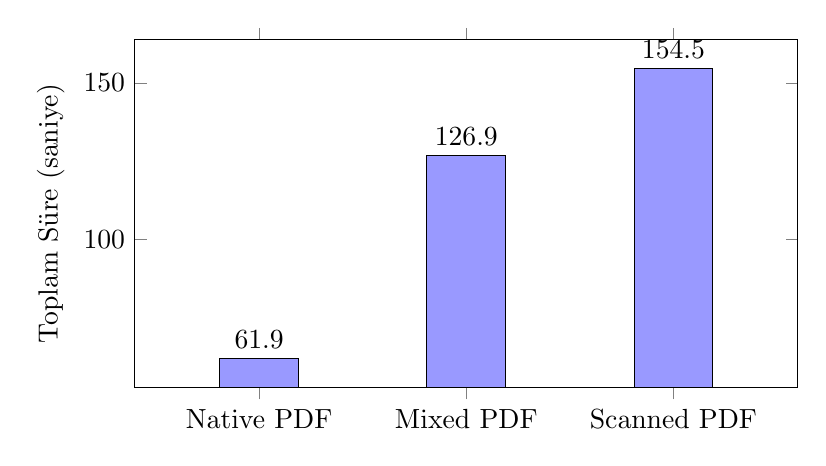
\begin{tikzpicture}
\begin{axis}[
    ybar,
    bar width=1cm,
    width=10cm,
    height=6cm,
    enlarge x limits=0.3,
    ylabel={Toplam Süre (saniye)},
    symbolic x coords={Native PDF, Mixed PDF, Scanned PDF},
    xtick=data,
    nodes near coords,
    nodes near coords align={vertical},
]
\addplot[fill=blue!40] coordinates {(Native PDF,61.9) (Mixed PDF,126.9) (Scanned PDF,154.5)};
\end{axis}
\end{tikzpicture}
\caption{Toplam Doküman İşleme Süreleri}
\end{figure}

\subsection{Doğruluk Metrikleri}
\begin{table}[H]
\centering
\caption{Doğruluk Analizi}
\begin{tabular}{ll}
\toprule
Metrik & Sonuç \\
\midrule
Tablo Çıkarım Başarısı & \%100 (4/4) \\
Pydantic Doğrulama & \%100 (3/3 test) \\
Doküman Tipi Tespiti & \%100 \\
VLM Skip Doğruluğu & Başarılı \\
\bottomrule
\end{tabular}
\end{table}

\needspace{16\baselineskip}
\section{Donanım Önerileri}

Mevcut sistemin kararlı çalışabilmesi için RAM bütçesi aşağıdaki gibi hesaplanmıştır:
\begin{itemize}[noitemsep]
\item phi4-mini: $\sim$2.8 GB
\item qwen2.5: $\sim$4.6 GB
\item qwen2.5vl: $\sim$6.0 GB (opsiyonel)
\item İşletim Sistemi + Docling: $\sim$4.0 GB
\item \textbf{Toplam (Tüm modeller): $\sim$17.4 GB}
\end{itemize}

\begin{table}[H]
\centering
\caption{Donanım İhtiyaçları ve Platform Karşılaştırması}
\resizebox{\textwidth}{!}{%
\begin{tabular}{lllll}
\toprule
Seviye & Donanım / İşlemci & Ekran Kartı (GPU) & RAM / VRAM & Notlar \\
\midrule
Minimum & Apple Silicon M1 & Tümleşik Metal GPU & 16 GB RAM & Dual model çalışır, VLM sınırlı \\
Önerilen & Apple M-Pro/Max & Tümleşik Metal GPU & 32 GB RAM & Tüm modeller aynı anda çalışır \\
PC İş İstasyonu & AMD Ryzen 9 / Threadripper & NVIDIA RTX 4080/4090 & 32--64GB RAM (16--24GB VRAM) & Windows/Linux, VLM dahil \%100 yerel \\
Kurumsal Sunucu & AMD EPYC / Intel Xeon & NVIDIA A10G / L4 / A100 & 64+ GB RAM (24--80GB VRAM) & Linux + vLLM ile yüksek throughput \\
\bottomrule
\end{tabular}%
}
\end{table}

\needspace{12\baselineskip}
\section{Maliyet Analizi}
Günde 1000 doküman işleme senaryosu baz alınarak yapılan maliyet tahmini aşağıdadır:

\begin{table}[H]
\centering
\caption{Cloud ve On-Premise Maliyet Karşılaştırması}
\begin{tabular}{lcc}
\toprule
Kalem & Cloud (Azure/OpenAI) & On-Premise \\
\midrule
Donanım Maliyeti & -- & $\sim$\$2.000 (tek seferlik Mac) \\
Aylık API Maliyeti & $\sim$\$3.000--\$5.000 & \$0 \\
1 Yıllık Toplam Maliyet (TCO) & $\sim$\$36.000--\$60.000 & $\sim$\$2.000 \\
Veri Gizliliği \& Güvenlik & Üçüncü taraf riski & \%100 Tam kontrol (Yerel) \\
Ölçeklenebilirlik & Sınırsız & Donanım kapasitesine bağlı \\
\bottomrule
\end{tabular}
\end{table}
\textit{Not: On-premise yatırımın donanım maliyeti genellikle sistemin devreye alındığı ilk ay içinde kendini amorti etmektedir (ROI).}

\section{Mimari Karar Kayıtları (ADR)}

\noindent \textbf{ADR-1: Docling Seçimi (vs Marker, MinerU, Unstructured):} Docling, layout analizi, tablo çıkarımı ve OCR entegrasyonunu tek pakette sunan yegane araçtır. BBox koordinatları sayesinde akıllı kırpma mümkün olmuştur. MIT lisansı ile ticari kullanıma uygundur.

\vspace{6pt}
\noindent \textbf{ADR-2: Çift LLM Mimarisi (vs Tek Model):} Tek model yaklaşımında (Qwen 2.5-VL), TTFT 157 saniyeyi buluyordu. Phi-4-mini'yi Phase 1'e atayarak ilk anlamlı veriyi 12.5 saniyeye düşürdük. Qwen 2.5'in derin analiz yeteneğinden de vazgeçmedik.

\vspace{6pt}
\noindent \textbf{ADR-3: Ollama Seçimi (vs vLLM, llama.cpp):} Ollama, macOS'ta sıfır yapılandırma ile çalışır, model yönetimi (pull/serve) kolaydır ve çoklu model desteği sunar. vLLM daha yüksek throughput sağlar ancak Linux + NVIDIA GPU gerektirir — production aşamasında değerlendirilecektir.

\vspace{6pt}
\noindent \textbf{ADR-4: Pydantic Şeması (vs JSON Schema / Free-form):} Pydantic v2, LLM çıktısını runtime'da doğrular ve tip uyumsuzluklarını otomatik düzeltir. Bu sayede parties listesindeki dict objelerinin string'e dönüştürülmesi gibi edge case'ler model değişikliği gerektirmeden çözülmüştür.

\section{Sınırlamalar ve Gelecek İyileştirmeler}

\subsection{Mevcut Sınırlamalar}
\begin{itemize}[noitemsep]
\item \textbf{İşlem süresi:} Native PDF'ler $\sim$62s, taranmış PDF'ler $\sim$155s sürmektedir. Bu sürelerin büyük bölümü LLM inference ve Docling parse aşamalarından kaynaklanmaktadır.
\item \textbf{Tek doküman işleme:} Sistem şu an sıralı (sequential) çalışmaktadır; batch processing veya kuyruk tabanlı işleme henüz uygulanmamıştır.
\item \textbf{Dil desteği:} Testler İngilizce dokümanlar üzerinde gerçekleştirilmiştir. Türkçe ve diğer dillerde doğruluk ayrıca test edilmelidir.
\item \textbf{Donanım bağımlılığı:} 16 GB RAM'de çift LLM + VLM aynı anda çalıştırılamaz; VLM kullanımı için 32 GB önerilir.
\end{itemize}

\needspace{8\baselineskip}
\subsection{Gelecek İyileştirmeler}
\begin{itemize}[noitemsep]
\item \textbf{Speculative Decoding:} Ollama/vLLM tarafında destek olgunlaştığında, küçük bir draft model ile 2-3x hız artışı hedeflenmektedir.
\item \textbf{vLLM ile Production Deployment:} Linux + NVIDIA GPU ortamında vLLM kullanılarak çok daha yüksek throughput ve eşzamanlı istek desteği sağlanabilir.
\item \textbf{Fine-tuning:} Kurum içi doküman tipleri (fatura, sözleşme, form) üzerinde LoRA tabanlı ince ayar yapılarak doğruluk artırılabilir.
\item \textbf{Batch Processing ve API:} REST API wrapper ve kuyruk tabanlı işleme ile çoklu doküman desteği eklenecektir.
\end{itemize}

\section{Sonuç}
Bu çalışma, açık kaynaklı LLM'ler kullanılarak tamamen on-premise çalışan bir doküman analizi çözümünün uygulanabilirliğini başarıyla kanıtlamıştır. Çift LLM Hibrit Mimarisi (Phi-4-mini + Qwen 2.5), tek model yaklaşımının kısıtlamalarını aşarak hız ile doğruluk arasında optimum dengeyi sağlamıştır.

Sisteme sağlanan üç farklı PDF formatı (native, scanned, mixed) sıfır veri kaybı ve \%100 şema uyumluluğuyla işlenmiştir. Akıllı VLM optimizasyonu ile gereksiz görsel işleme ortadan kaldırılmış, model swap eliminasyonu ile phase geçiş gecikmeleri minimize edilmiştir.

On-premise yaklaşım, bulut çözümlerine kıyasla veri gizliliği, düşük maliyet (1 yıllık TCO farkı $\sim$34,000--58,000) ve tam kontrol avantajları sunmaktadır. Mevcut PoC, production ortamına taşınmaya hazır bir temel oluşturmaktadır.

\end{document}
